\documentclass[border=0pt]{standalone}

\usepackage{tikz}
\usepackage{pgfplots}
\usepackage{pgfplotstable}
\pgfplotsset{compat=newest}
\usepgfplotslibrary{groupplots}
\usetikzlibrary{pgfplots.groupplots}
\usepackage{filecontents}

%\renewcommand{\rmdefault}{phv}
%\renewcommand{\sfdefault}{phv}
%\usepackage[helvet]{sfmath}


%%%%% TIKZ %%%%%
\usepackage{tikz}
\usetikzlibrary{arrows}
\usetikzlibrary{decorations.pathreplacing} 
\usetikzlibrary{decorations.markings}
\newcommand{\midarrow}{\tikz \draw[-triangle 60] (0,0) -- +(.08,0);}

\tikzset{
	null/.style={
		text width=0.5cm,
		minimum height=0.5cm,
		text centered,
	},
	latent/.style={
		circle,
		draw=black, 
		thick, 
		text width=0.5cm,
		minimum height=0.5cm,
		text centered, 
	}, 
	manifest/.style={
		rectangle,
		draw=black, 
		thick, 
		text width=0.5cm,
		minimum height=0.5cm,
		text centered, 
	}, 	
	arrow/.style={
		->, 
		thick,
	},
}
%%%%% PGF PLOTS %%%%%%


\begin{document}
\mbox{

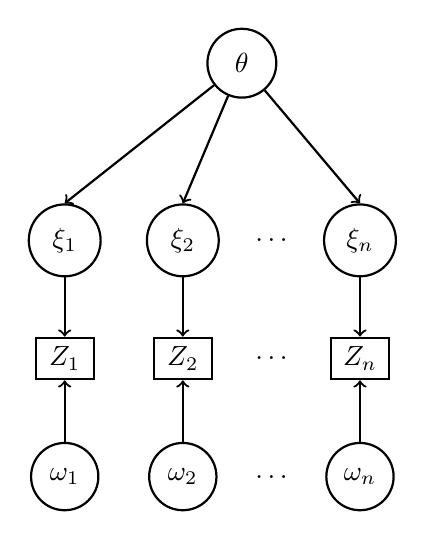
\begin{tikzpicture}
		\newcommand{\dx}{1.5cm}
		\newcommand{\dy}{1.5cm}

		
		% VAF latent variable 
		\node[latent] (vaf) at (1.5*\dx, 1.5*\dy) {$\theta$} ; 
		
		% Latent variables 
		\node[latent] (xi1) at (0,0) {$\xi_1$} ; 
		\node[latent] (xi2) at (\dx,0) {$\xi_2$} ; 
		\node[null] (xi_null) at (1.75*\dx,0) {$\dots$} ; 
		\node[latent] (xik) at (2.5*\dx,0) {$\xi_n$} ; 

		% X observations
		\node[manifest] (x1) at (0,-\dy) {$Z_1$} ; 
		\node[manifest] (x2) at (\dx,-\dy) {$Z_2$} ; 
		\node[null] (x_null) at (1.75*\dx,-\dy) {$\dots$} ; 
		\node[manifest] (xk) at (2.5*\dx,-\dy) {$Z_n$} ; 
			
		\node[latent] (o1) at (0,-2*\dy) {$\omega_1$} ; 
		\node[latent] (o2) at (\dx,-2*\dy) {$\omega_2$} ; 
		\node[null] (o_null) at (1.75*\dx,-2*\dy) {$\dots$} ; 
		\node[latent] (ok) at (2.5*\dx,-2*\dy) {$\omega_n$} ; 
			
		\draw[arrow] (vaf) -- (xi1.north) ; 
		\draw[arrow] (vaf) -- (xi2.north) ; 
		\draw[arrow] (vaf) -- (xik.north) ; 
		
		\draw[arrow] (xi1.south) -- (x1.north) ;  
		\draw[arrow] (xi2.south) -- (x2.north) ;  
		\draw[arrow] (xik.south) -- (xk.north) ; 
			
		\draw[arrow] (o1.north) -- (x1.south) ;  
		\draw[arrow] (o2.north) -- (x2.south) ; 
		\draw[arrow] (ok.north) -- (xk.south) ; 


	\end{tikzpicture}
% Add tikz here!
}
\end{document}
